
\section{Model-based Analysis}

As described in the introduction, prefetching has the potential to enable visualization systems to respond with interactive latencies.  However, current approaches are designed for interfaces with limited options for user interaction~\cite{}; many have suggested that increasing the expressivity of the interface (e.g., the number of possible user actions) makes the prediction task significantly more challenging.  In this section, we seek to understand the minimum accuracy for model needs in order to support low user perceived latencies, as well as the conditions that affect this accuracy.

\subsection{The Model}

Our goal is to estimate the minimum prediction accuracy $\alpha$ needed in order to ensure that the user perceived latency $l_{user}$ is below a fixed threshold (e.g. 100ms~\cite{} or 500ms).
Let $T=0$ be the time.
We assume that the user will perform her request at $T=t$ where $t \ge 0$, and that the cost of answering a request consists of fetching and rendering the results.
$l_{user}$ is defined as the time between $t$ and the change reflected in the visualization. 
Let $l_{net}$ be the latency to execute a request, transfer the results across the network, and render it on screen.   In a typical system, $l_{user} = l_{net}$, which can be undesirable when query processing or the network latency are high.
Prefetching allows the client to proactively answer a request at $T=0$ and store the results in a client cache.
If a future request accessed data in the cache, then it can take much less time $l_{cache} < l_{net}$ and result in a more responsive user perceived experience.

We now model the expected user perceived latency as $l_{cache} + max(0, l_{net} - t)$ if model accurately predicted the request, and $l_{net}$ if it mispredicted.  The $max()$ operation accounts for cases when the cost of a cache miss is larger than $t$:
$$l_{user} = (l_{cache} + max(0, l_{net}-t))\times \alpha + l_{net}\times(1-\alpha) $$
Rearranging the terms, we can derive the minimum prediction accuracy in order to maintain $l_{user}$.
%$$\alpha = \frac{l_{net} - l_{user}}{l_{net} - l_{cache}}$$
$$\alpha = \frac{l_{user} - l_{net}}{l_{cache} + max(0, l_{net}-t) - l_{net}}$$

\ewu{Describe common constants} 
Figure~\ref{fig:model_base} plots the model accuracy for two commonly cited $l_{user}$ thresholds (100 and 500ms).  The x-axis varies $l_{net}$ and each line represents the percentage of the prefetching costs that the user will experience.  For instance, when $\frac{t}{l_{net}}=1$, the user initiates the request at $T=t=l_{net}$ and does not experience any of the prefetching costs, whereas when $\frac{t}{l_{net}}=0.5$, the prefetching request is only half complete by the time the user initiates her request at $T=0.5\times l_{net}$.
\ewu{Describe the figure}

\begin{figure}[ht]
	\centering
	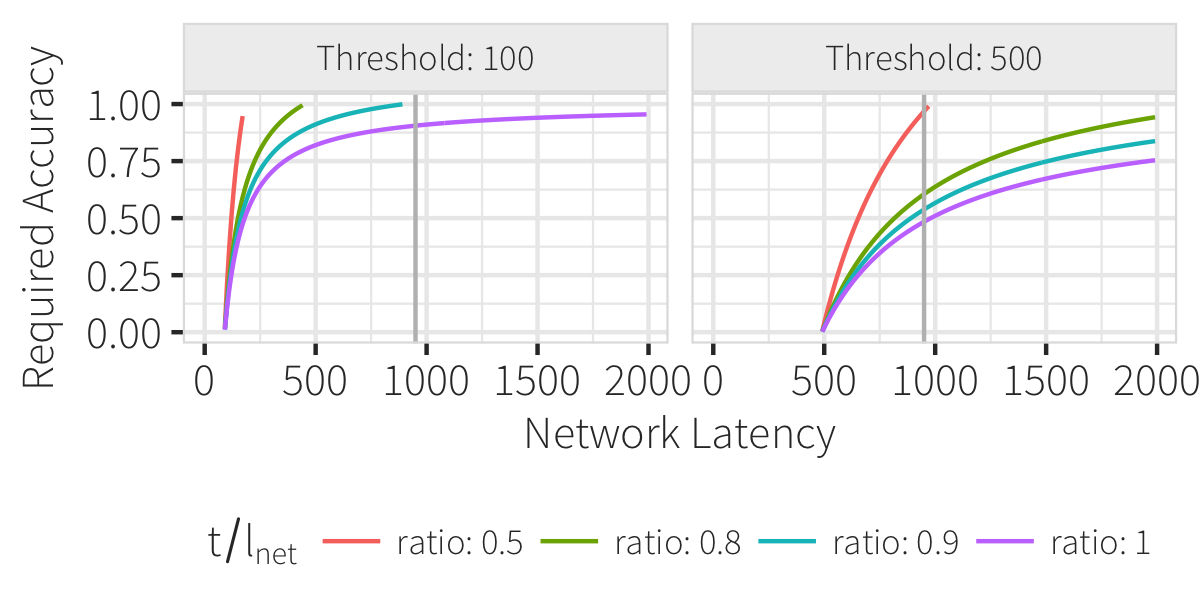
\includegraphics[width=1\columnwidth]{figures/model_base}
 	\caption{Minimum $\alpha$ vs network latency (x-axis), $\frac{t}{l_{net}}$ ratios (lines), and two thresholds (facets).}
    \label{fig:model_base}
\end{figure}



\stitle{Vary Prefetch Concurrency}
Most modern data processing systems are able to execute multiple concurrent requests~\cite{ebenstein2016fluxquery,giannikis2012shareddb}.  
We now vary the number of concurrent prefetch requests $N$;
the $(1-\alpha)^N$ term is the probability that none of the prefetch requests match the user's actual request at $T=t$:
%
$$l_{user} = (l_{cache} + max(0, l_{net} - t)\times (1-(1-\alpha)^N) + l_{net}\times(1-\alpha)^N $$
%
Rearranging the terms results in the following minimum prediction accuracy:
%
$$\alpha = 1 - \left(\frac{l_{cache}+max(0,l_{net}-t)-l_{user}}{max(0,l_{net}-t)-l_{net}}\right)^{1/N}$$

\begin{figure}[h]
	\centering
	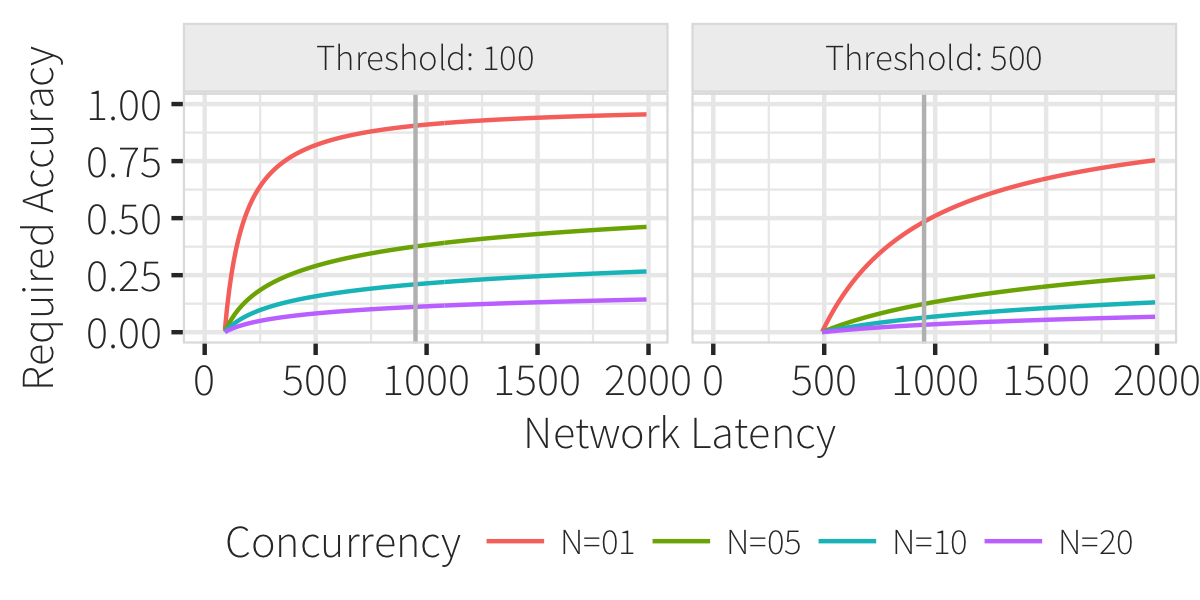
\includegraphics[width=1\columnwidth]{figures/model_concurrency}
 	\caption{Minimum $\alpha$ vs network latency (x-axis), concurrency (lines), and two latency thresholds (facets).}
  \label{fig:model_concurrency}
\end{figure}


Figure~\ref{fig:model_concurrency} shows that increasing the number of concurrent requests has an immediate effect on $\alpha$ ($t=l_{net}$ in these plots).    With $N=20$, a prediction model need only be $12\%$ accurate to ensure an interactive latency of $l_{user}=100$, while ensuring  $l_{user}=500$ only requires an accuracy of $3.5\%$. \ewu{Describe implications}


\stitle{Network Latency Variance}
Figure~\ref{fig:model_std} simulates $l_{net}$ drawn from a gaussian distribution with standard deviation of $0, 100, 500$ milliseconds.  We set $N=20$, $t=l_{net}$.  We find that although the request variance affects the required model accuracy when $l_{net}$ is low, the curves converge to similar points as $l_{net}$ increases, irrespective of the variance.

\begin{figure}[h]
	\centering
	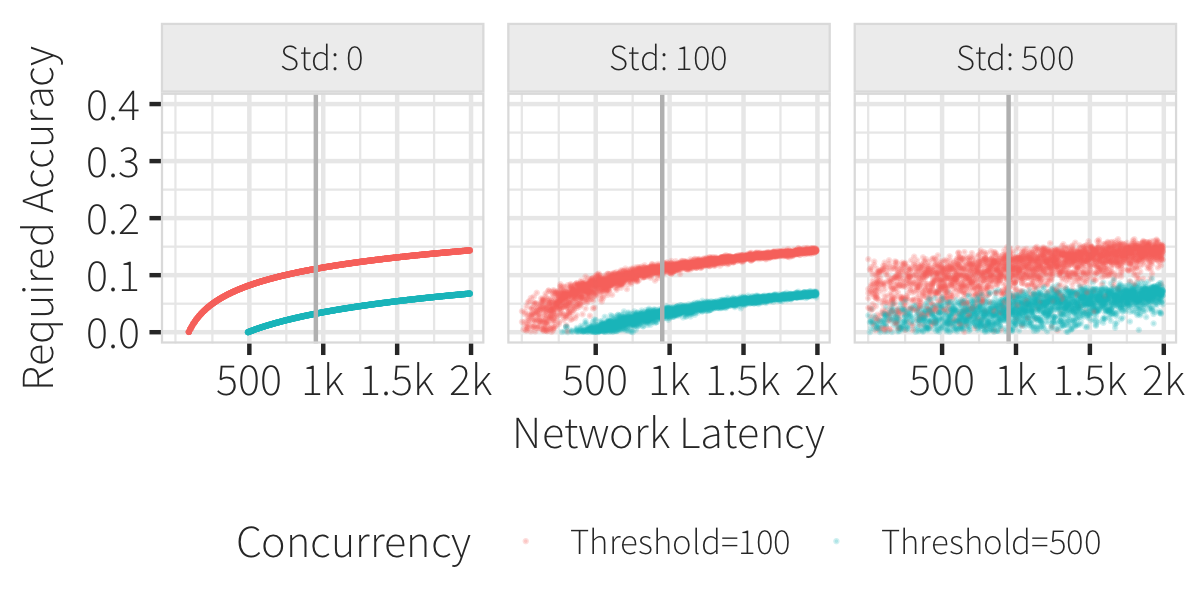
\includegraphics[width=1\columnwidth]{figures/model_std}
 	\caption{Minimum $\alpha$ vs network latency (x-axis), concurrency (lines), and two latency thresholds (facets).}
  \label{fig:model_std}
\end{figure}

\begin{figure}[hb]
	\centering
	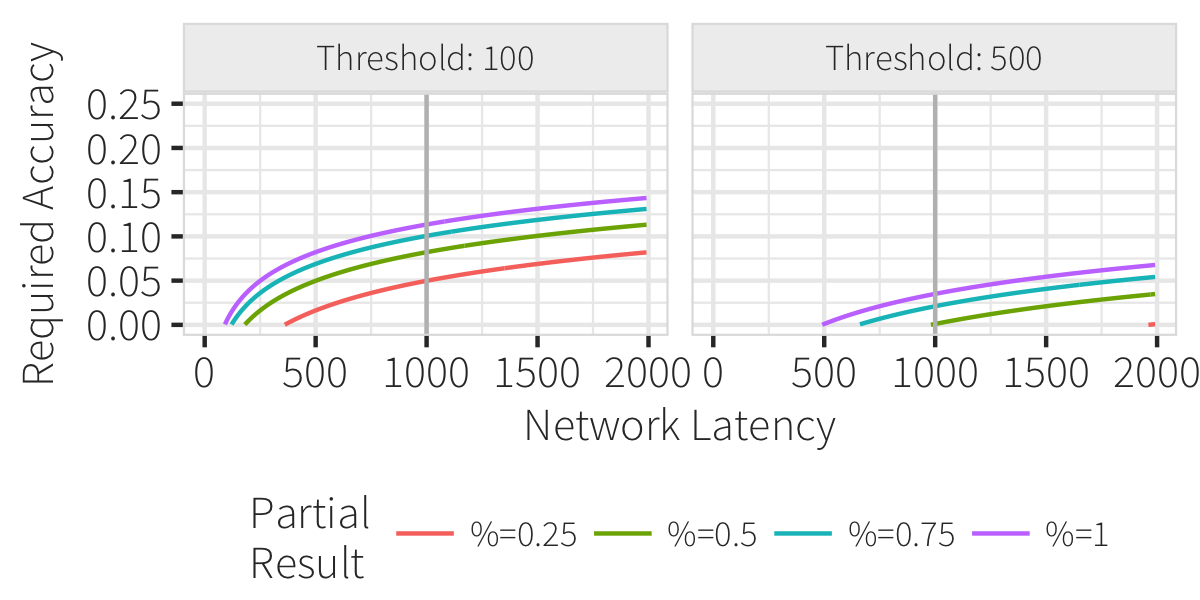
\includegraphics[width=1\columnwidth]{figures/model_partial}
 	\caption{Required prediction accuracy as a function of network latency, under progressive conditions where partial responses are sufficient.}
    \label{fig:model_partial}
\end{figure}


\stitle{Progressive Loading}
\ewu{Lots of work on approximation and perceptual inaccuracy.}  In our final analysis, we simulate the effects of partial results by simply reducing the time it takes to respond to a request.
A powerful result is that combining concurrency and partial results can reduce the required accuracy of the prediction model to nearly $0$ and still support interactivity of $l_{user}=500ms$ when $l_{net}\le 2000$.






\subsection{Discussion}

\ewu{Argue that it is clear that progressive encoding and apprximate results will be the future.  Thus the combination of partial results and concurrency go hand in hand.  We also see that the prediction model simply needs to be ``good enough'' with an accuracy around $10\%$.  When the number of possible interactions are limited, then a random model is sufficient.  However when it is unlimited, then the accuracy can easiry be very low~\cite{}.  }



Assuming a tile is XXX kilobytes, and a throughput of $T mb/s$, then can sustain a concurrency level of XXX.  
When combined with progressive loading of $20\%$ (base this number off sampling and immens arguments), increases the concurrency level to XXX, 
and the model accuracy to YYY.  In many existing settings, where the number of interaction options is limited, this effectively means the prediction model
can draw randomly and be effective.  


However, in interfaces such as XXX, the number of possible interactions are roughly YYY, for which existing techniques would fail.  Under our analysis, the model simply needs to be.

